\section{Introduction}


\rem{
\begin{frame}
 
 \only<1>{

   \heading{{\color{red}\bf ode}int}

   \vspace{6ex}

   \Large

   ode \hspace{4ex} ordinary differential equation

   \vspace{5ex}

}

 \only<2>{
   \heading{ode{\color{red}\bf int}}

   \vspace{6ex}

   \Large

   ode \hspace{4ex} ordinary differential equation

   \vspace{3ex}

   int \hspace{4ex} integration
}

\end{frame}
}


\begin{frame}
 
\heading{What is an ODE? -- Examples}

\vspace{2ex}

\begin{minipage}{0.48\textwidth}
 \begin{center}
  Newtons equations

  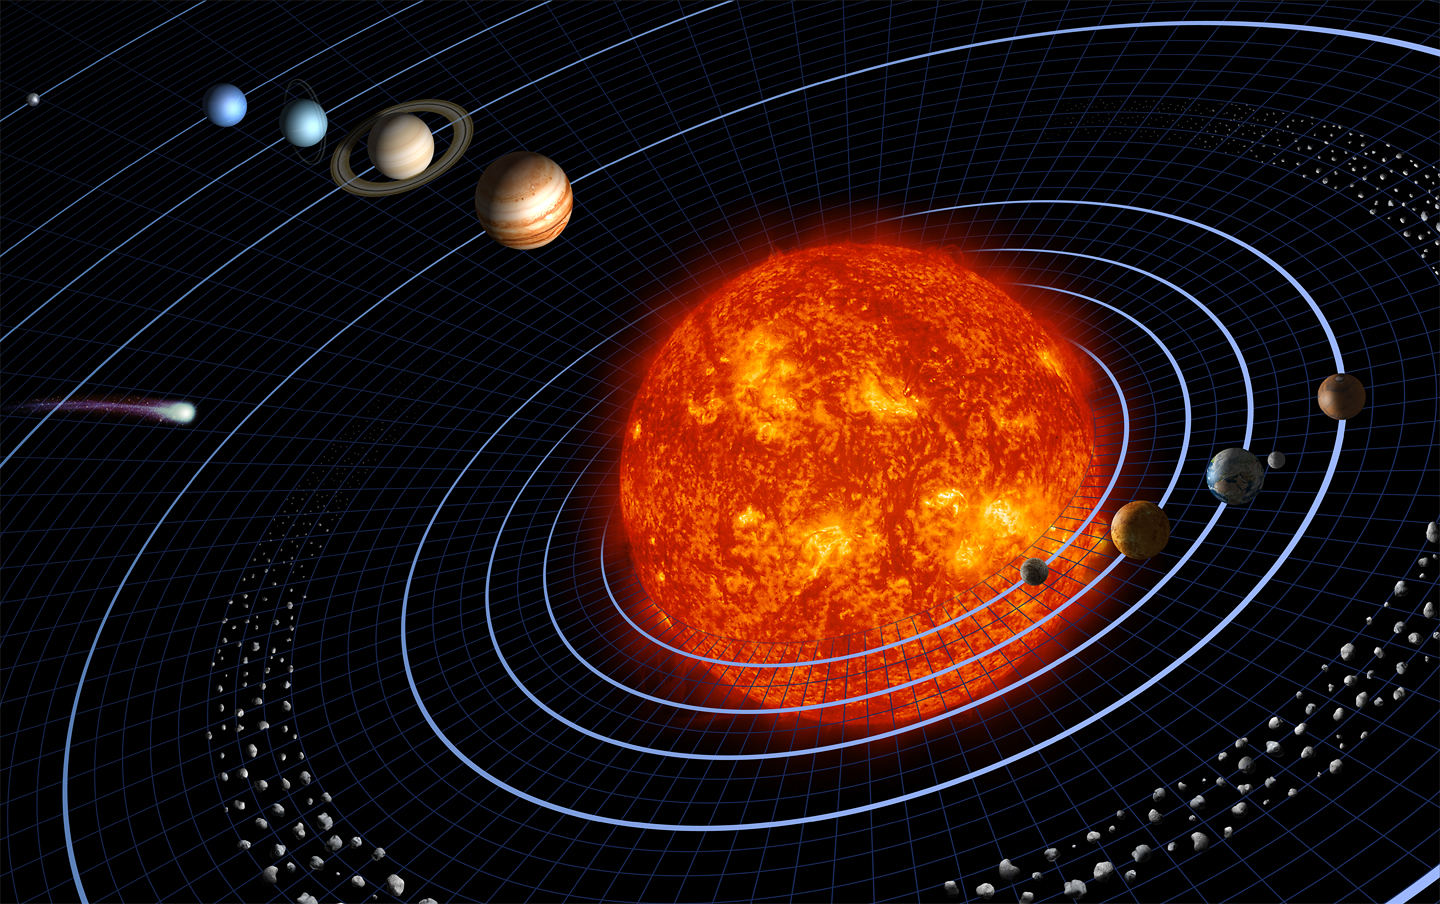
\includegraphics[draft=false,width=0.8\textwidth]{solar_system.jpg}
 \end{center}
\end{minipage}
% \pause
\begin{minipage}{0.48\textwidth}
 \begin{center}
  Reaction and relaxation equations (i.e. blood alcohol content, chemical reaction rates)
 \end{center}
\end{minipage}
% \pause
\vspace{2ex}

\begin{minipage}{0.48\textwidth}
 \begin{center}
  Granular systems

  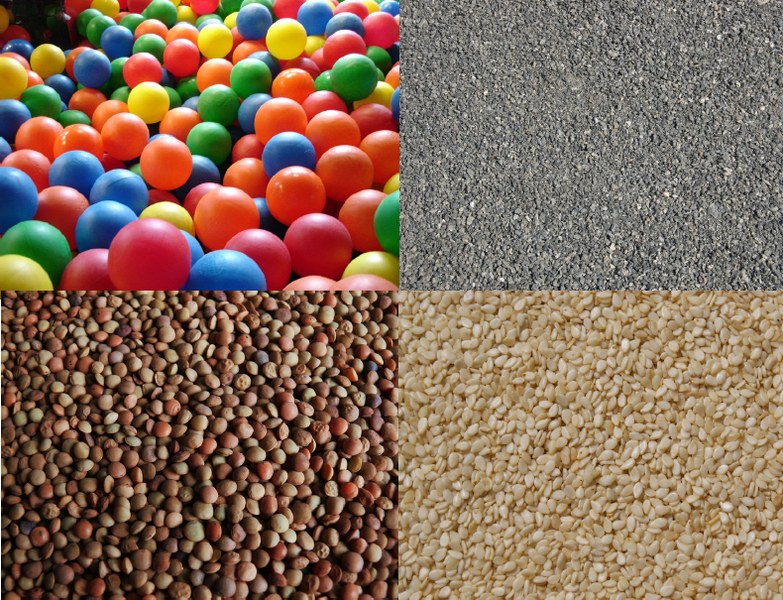
\includegraphics[draft=false,width=0.65\textwidth]{granular_system.png}
 \end{center}
\end{minipage}
% \pause
\begin{minipage}{0.48\textwidth}
 \begin{center}
  Interacting neurons

  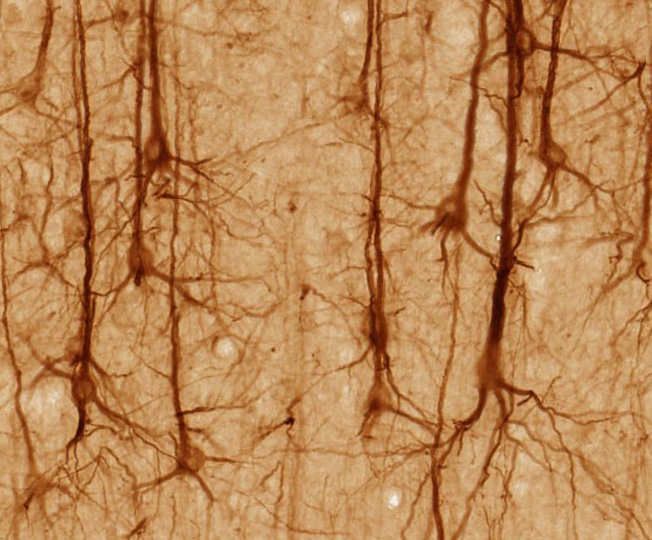
\includegraphics[draft=false,width=0.6\textwidth]{neuron.jpg}
 \end{center}
\end{minipage}
% \pause
\vspace{2ex}

\begin{itemize}
 \item Many examples in physics, biology, chemistry, social sciences
 \item Fundamental in mathematical modelling
\end{itemize}

\end{frame}



\begin{frame}
 
 \heading{What is an ODE?}

 $$\frac{\de x(t)}{\de t} = f\big(x(t) , t\big) \qquad \qquad {\scriptsize \text{short form}} \qquad \dot{x} = f(x,t)
$$

 \begin{itemize}
  \item $x(t)$ -- dependent variable
  \item $t$ -- indenpendent variable (time)
  \item $f(x,t)$ -- defines the ODE
 \end{itemize}

\vspace{4ex}

 Initial Value Problem (IVP):

 $$\dot x = f( x , t ) ,\qquad x(t=0) = x_0$$

\end{frame}


\begin{frame}
  
 \heading{Numerical integration of ODEs}
  
\vspace{4ex}
    Find a numerical solution of an ODE and its IVP
    \[ \dot{x} = f(x,t) \,\,\textrm{,} \quad \quad x(t=0) = x_0\]

   \vspace{2ex}

   Example: Explicit Euler
   \[ x(t + \Delta t ) = x(t) + \Delta t \,\cdot\, f(x(t),t) + \mathcal{O}(\Delta t^2)\]

   \vspace{2ex}

   General scheme of order $s$
    \[ x(t) \,\, \mapsto \,\, x(t+\Delta t) \quad \quad \text{, or}\]
    \[x(t + \Delta t) = \mathcal{F}_t x(t) + \mathcal{O}(\Delta t^{s+1})\]

\end{frame}




\frame{
%  \frametitle{odeint - Solving ODEs in C++}

\heading{\bf \color{red}odeint}

\vspace{2ex}

\centerline{Solving ordinary differential equations in C++}

\vspace{2ex}

Open source
\begin{itemize}
\item Boost license -- do whatever you want do to with it 
\item Accepted as Boost library -- Release with Version 1.53
\end{itemize}

% \pause

\vspace{2ex}

Download
\begin{itemize}
\item \texttt{\textbf{www.odeint.com}}
\end{itemize}

% \pause

\vspace{2ex}

Modern C++
\begin{itemize}
 \item Paradigms: generic, template-meta programming, functional
 \item Fast, easy-to-use and extendable.
 \item Container independent
 \item Portable
\end{itemize}

}



\begin{frame}
 \heading{Structure of \odeint}
 
 \vspace{2ex}
 \centerline{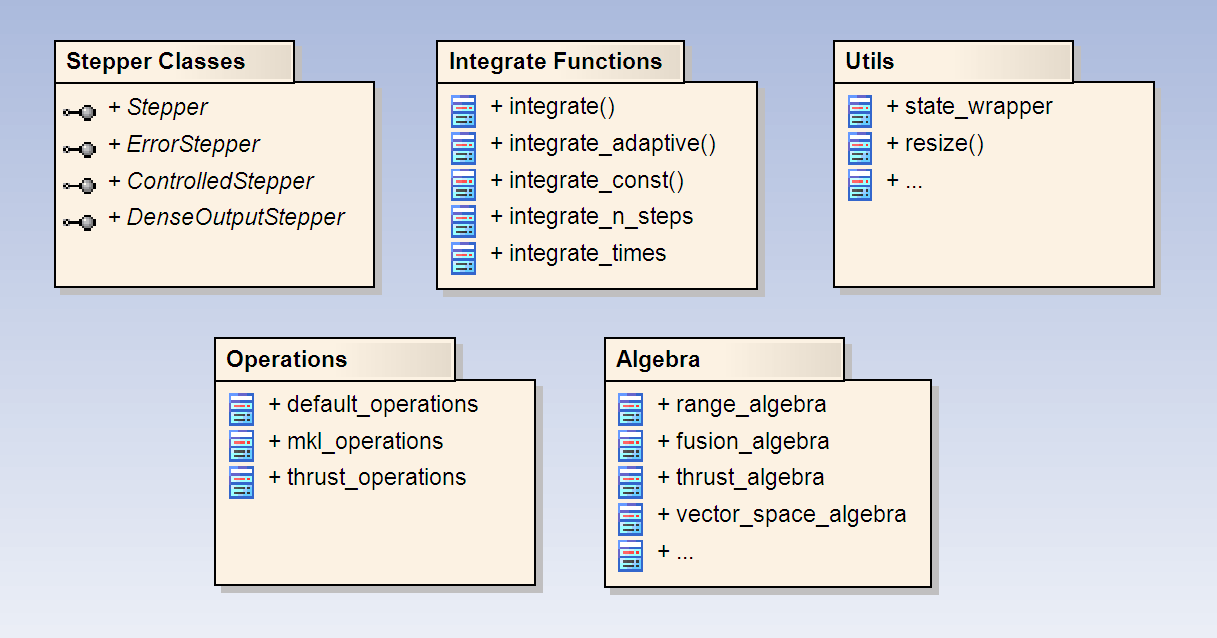
\includegraphics[draft=false,width=1.0\textwidth]{odeint_components.png}}

\end{frame}




\begin{frame}[fragile]
 \heading{Motivation}

 \vspace{2ex}

 We want to solve ODEs $\dot{x}=f(x,t)$
 \begin{itemize}
  \item using  {\tt double}, {\tt std::vector}, {\tt std::array}, \dots as state types.
  \item with complex numbers,
  \item on one, two, three-dimensional lattices, and or on graphs.
  \item on graphic cards.
  \item with arbitrary precision types.
 \end{itemize}

 \vspace{2ex}

Existing libraries support only one state type!

\vspace{4ex}
\centerline{\textbf{Container independent} and {\bf portable} algorithms are needed!}

\end{frame}







\rem{
\begin{frame}
  \heading{Motivation: The interface problem in C/C++, SKIP!!}

  \vspace{2ex}
  
    \begin{itemize}
      \item Many frameworks exist to do numerical computations.
      \item Data has to be stored in containers or collections.
      \item GSL: {\tt gsl\_vector}, {\tt gsl\_matrix}
      \item NR: pointers with Fortran-style indexing
      \item Blitz++, MTL4, boost::ublas
      \item QT: {\tt QVector}, wxWidgets: {\tt wxArray}, MFC: {\tt CArray}
    \end{itemize}

  %\vspace{2ex}

    {\bf \color{red} But:} All books on C++ recommend the use of the STL containers {\tt std::vector},
    {\tt std::list}, \dots

 \pause

  %\vspace{2ex}

  \begin{block}{Theoretical solution of the interface mess}
  GoF Design Pattern: Adaptor, also known as Wrapper
  \end{block}

  \pause

  \begin{exampleblock}{Alternative}
   Generic, container independent algorithms
  \end{exampleblock}

\end{frame}
}



\rem{
\begin{frame}
  
  \heading{Portability of your algorithm, SKIP!!}

  \vspace{1ex}

  How to run your algorithm?
    \begin{itemize}
      \item Single machine, single CPU
      \item Single machine, multiple CPU's (OpenMP, threads, ...)
      \item Multiple machines (MPI)
      \item GPU (Cuda, Thrust, OpenCL)
    \end{itemize}

  \pause

  \vspace{1ex}

  Which data types are used by your algorithm?
   \begin{itemize}
    \item Build-in data types -- \texttt{double}, \texttt{complex<double>}
    \item Arbitrary precision types -- GMP, MPFR
    \item Vectorial data types \texttt{float2d}, \texttt{float3d}
   \end{itemize}

  \pause

  \vspace{1ex}

  \begin{block}{Theoretical solution}
    GoF Design Pattern: Strategy, also known as Policy
  \end{block}

  \begin{exampleblock}{Alternative}
   Generic algorithms
  \end{exampleblock}

\end{frame}
}











\begin{frame}[fragile]

\heading{Example -- Pendulum}

\vspace{2ex}

\begin{columns}[T]
  \begin{column}{0.35\textwidth}
    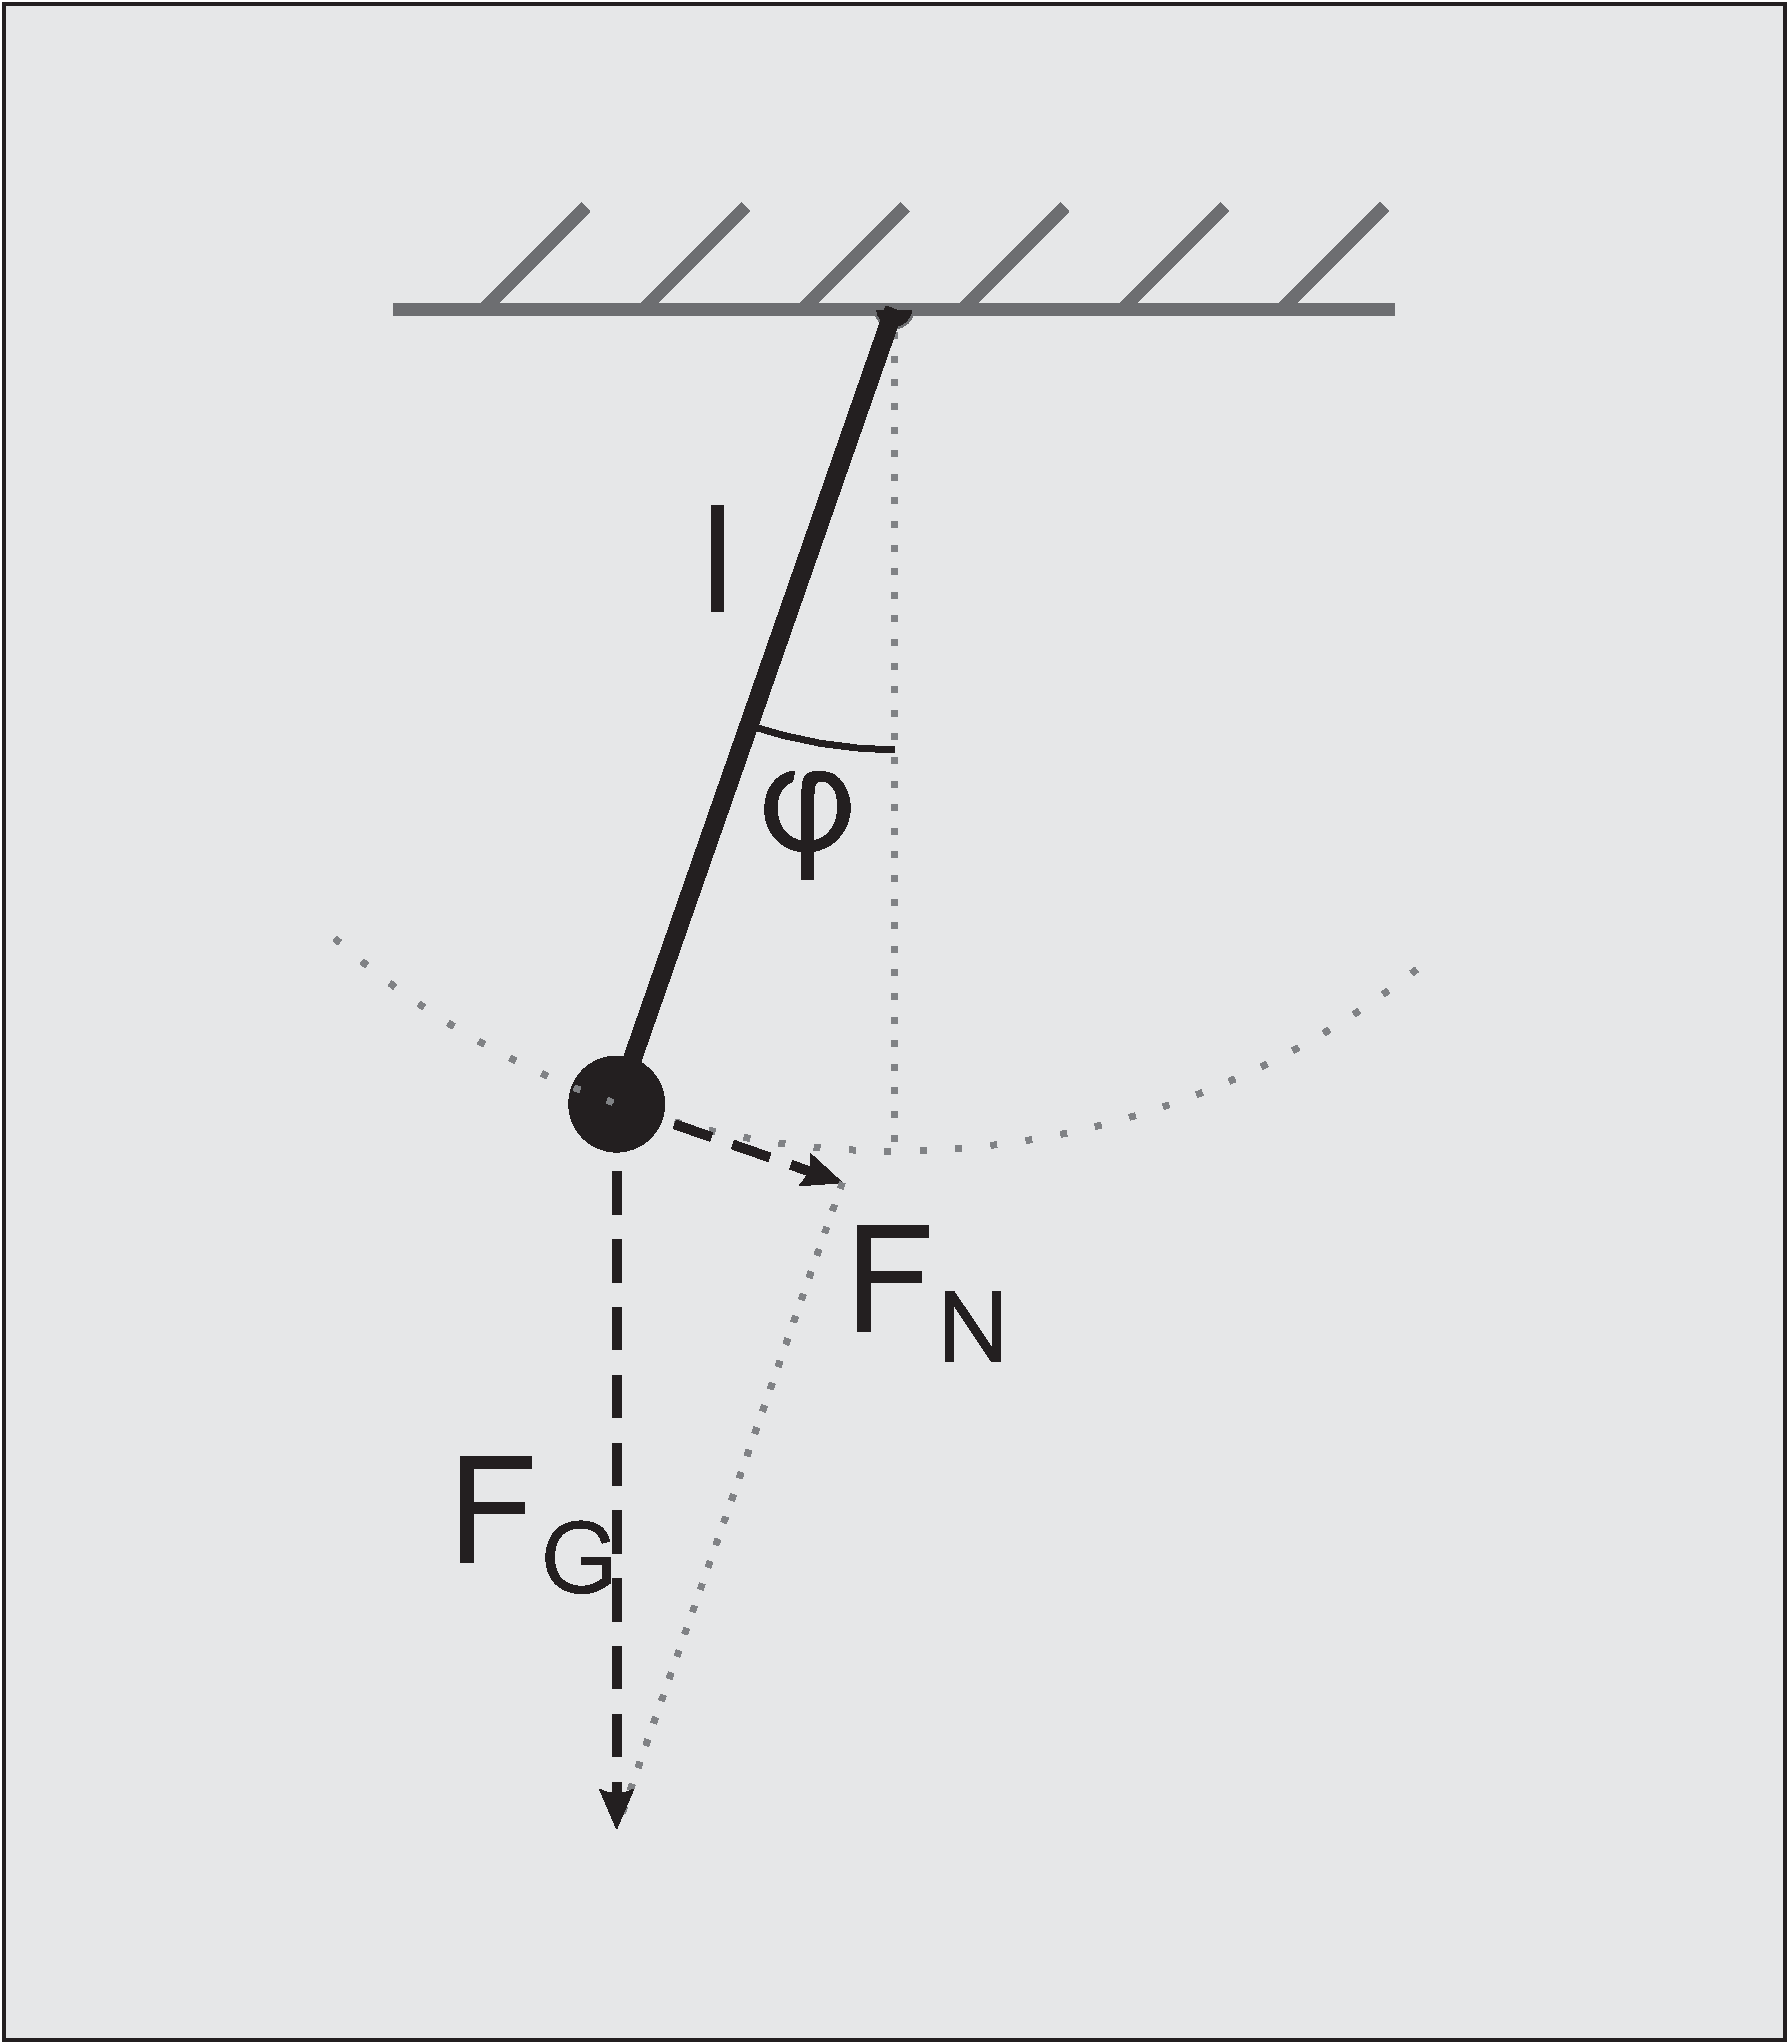
\includegraphics[draft=false,width=1.0\textwidth]{pendulum.pdf}

   \vspace{4ex}
  \end{column}

  \begin{column}{0.65\textwidth}

 $$\ddot{\varphi} = -\omega_0^2 \sin \varphi - \mu \dot{\varphi} + \varepsilon \sin \omega_E t $$

 \vspace{2ex}

 Create a first order ODE

 \vspace{1ex}

 \centerline{$x_1 = \varphi \,\, \text{,} \quad x_2 = \dot{\varphi}$}

 \vspace{-3ex}
 \begin{align*}
   \dot{x_1} &= x_2 \\
   \dot{x_2} &= - \omega_0  \sin x_1 - \mu x_2 + \varepsilon \sin \omega_E t  
 \end{align*}


 $x_1$ and $x_2$ are the state space variables

 
  \end{column}
\end{columns}

 

\end{frame}







\begin{frame}[fragile]

\centerline{ \Large Let's solve the pendulum example numerically}

\vspace{2ex}
\begin{lstlisting}
#include <boost/numeric/odeint.hpp>

namespace odeint = boost::numeric::odeint;
\end{lstlisting}

\vspace{2ex}

\centerline{$\dot{x_1} = x_2 \,\,\text{,} \quad \dot{x_2} = - \omega_0 \sin x_1 - \mu x_2 + \varepsilon \sin \omega_E t$}

\vspace{2ex}
\begin{lstlisting}
typedef std::array<double,2> state_type;
\end{lstlisting}

\end{frame}

\begin{frame}[fragile]

\centerline{ \Large Let's solve the pendulum example numerically}

\vspace{2ex}

$\dot{x_1} = x_2$, $\dot{x_2} = - \omega_0^2 \sin x_1 - \mu x_2 + \varepsilon \sin \omega_E t$ \hspace{6ex} $\omega_0^2 = 1$

\vspace{2ex}

\begin{lstlisting}
struct pendulum
{
  double m_mu, m_omega, m_eps;

  pendulum(double mu,double omega,double eps)
  : m_mu(mu),m_omega(omega),m_eps(eps) { }

  void operator()(const state_type &x,state_type &dxdt,double t) const
  {
    dxdt[0] = x[1];
    dxdt[1] = -sin(x[0]) - m_mu * x[1] +
        m_eps * sin(m_omega*t);
  }
};
\end{lstlisting}

\end{frame}

\begin{frame}[fragile]
 \centerline{ \Large Let's solve the pendulum example numerically}

\vspace{2ex}
$\varphi(0) = x_1(0) = 1 \,\, \text{,} \quad \dot{\varphi}(0) = x_2(0) = 0$
\vspace{2ex}

\begin{lstlisting}
odeint::runge_kutta4< state_type > rk4;
state_type x = {{ 1.0 , 0.0 }};
double t = 0.0 , t_end = 10.0 , dt = 0.0;
integrate_const( rk4 ,
    pendulum( 0.1 , 1.05 , 1.5 ) ,
    x , t , t_end , dt ,
    []( const state_type &x , double t ) {
        cout << x[0] << " " << x[1] << "\n"; }
    );
\end{lstlisting}

\vspace{2ex}

\centerline{$x(0) \mapsto x(\Delta t) \mapsto x(2\Delta t) \mapsto x(3\Delta t) \mapsto \dots$}

\end{frame}



\rem{
\begin{frame}[fragile]
 \heading{Simulation}

 \vspace{1ex}

 \centerline{Oscillator: $\mu=0 \,\, \text{,} \quad \omega_E = 0 \,\, \text{,} \quad \varepsilon=0$}

 \vspace{1ex}

 \centerline{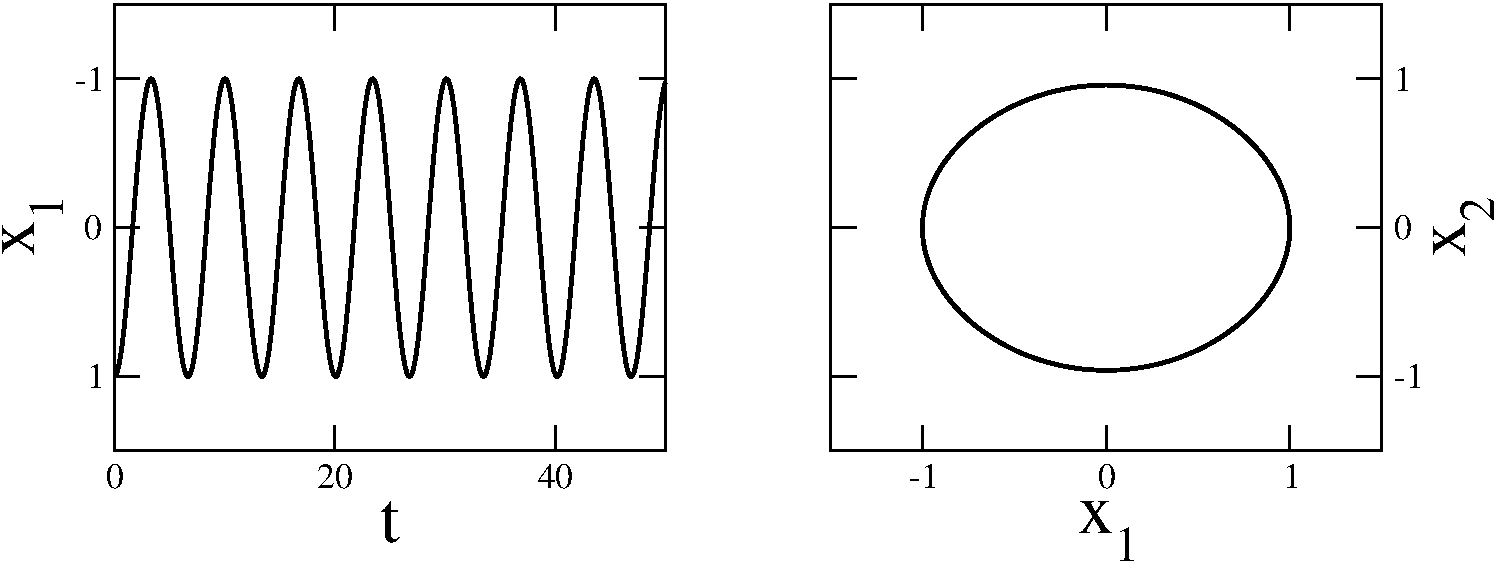
\includegraphics[draft=false,width=0.6\textwidth]{undamped.pdf}}

% \vspace{1ex}
 
\centerline{Damped oscillator: $\mu=0.1 \,\, \text{,} \quad \omega_E = 0 \,\, \text{,} \quad \varepsilon=0$}

 \vspace{1ex}

 \centerline{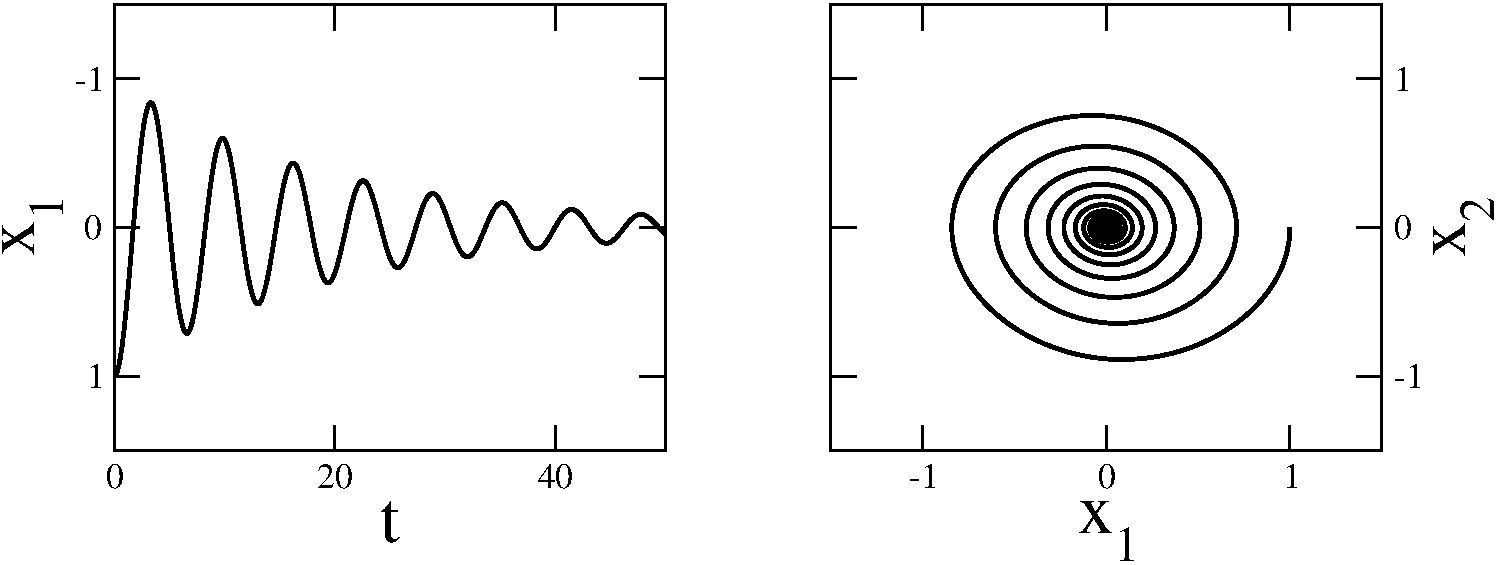
\includegraphics[draft=false,width=0.6\textwidth]{damped.pdf}}

% \vspace{1ex}

 \centerline{Damped, driven oscillator: $\mu=0.1 \,\, \text{,} \quad \omega_E = 1.05 \,\, \text{,} \quad \varepsilon=1.5$}

 \vspace{1ex}

 \centerline{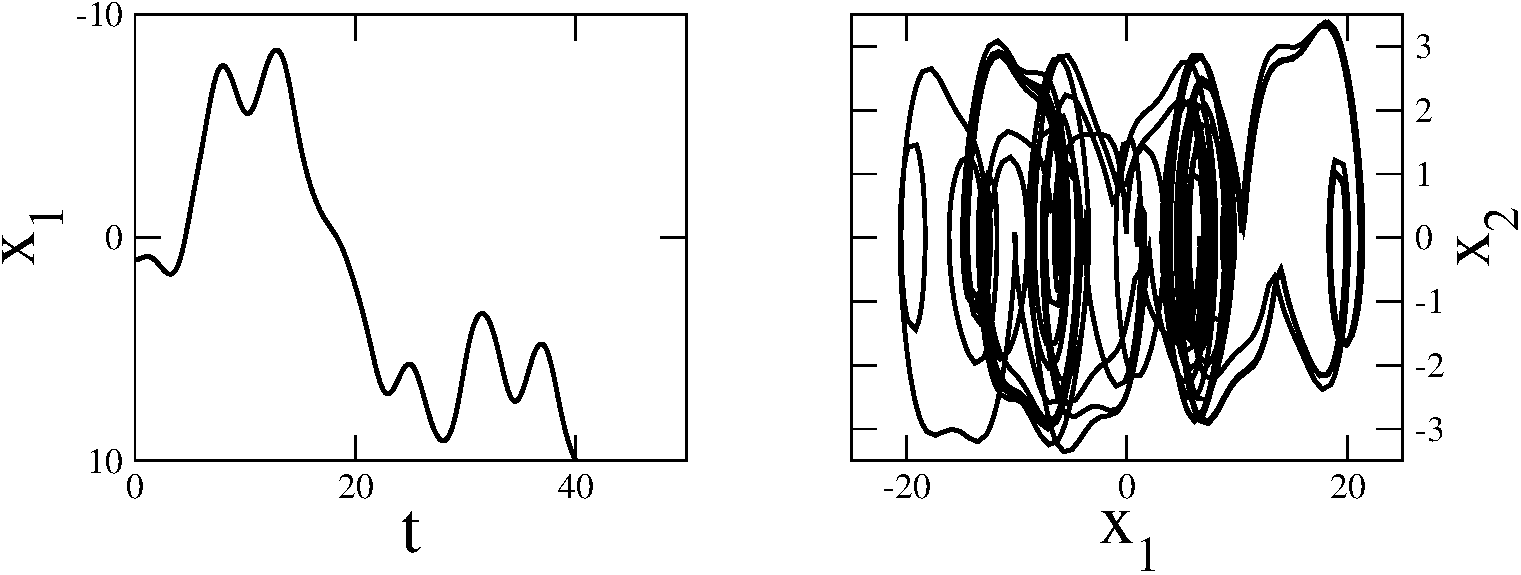
\includegraphics[draft=false,width=0.6\textwidth]{damped_driven.pdf}}


\end{frame}
}





\begin{frame}[fragile]
 \heading{Simulation}

 \vspace{2ex}

\begin{minipage}[t]{0.5\textwidth}
\vspace{0pt}
Oscillator

\vspace{1ex}
$\mu=0 \, \text{,} \,\, \omega_E = 0 \, \text{,} \,\, \varepsilon=0$

\vspace{7ex}
Damped oscillator:

\vspace{1ex}
$\mu=0.1  \, \text{,} \,\, \omega_E = 0  \, \text{,} \,\, \varepsilon=0$

\vspace{7ex}
Damped, driven oscillator:

\vspace{1ex}
$\mu=0.1  \, \text{,} \,\, \omega_E = 1.05  \, \text{,} \,\, \varepsilon=1.5$
\end{minipage} %\pause
\begin{minipage}[t]{0.49\textwidth}
\vspace{0pt}
\centerline{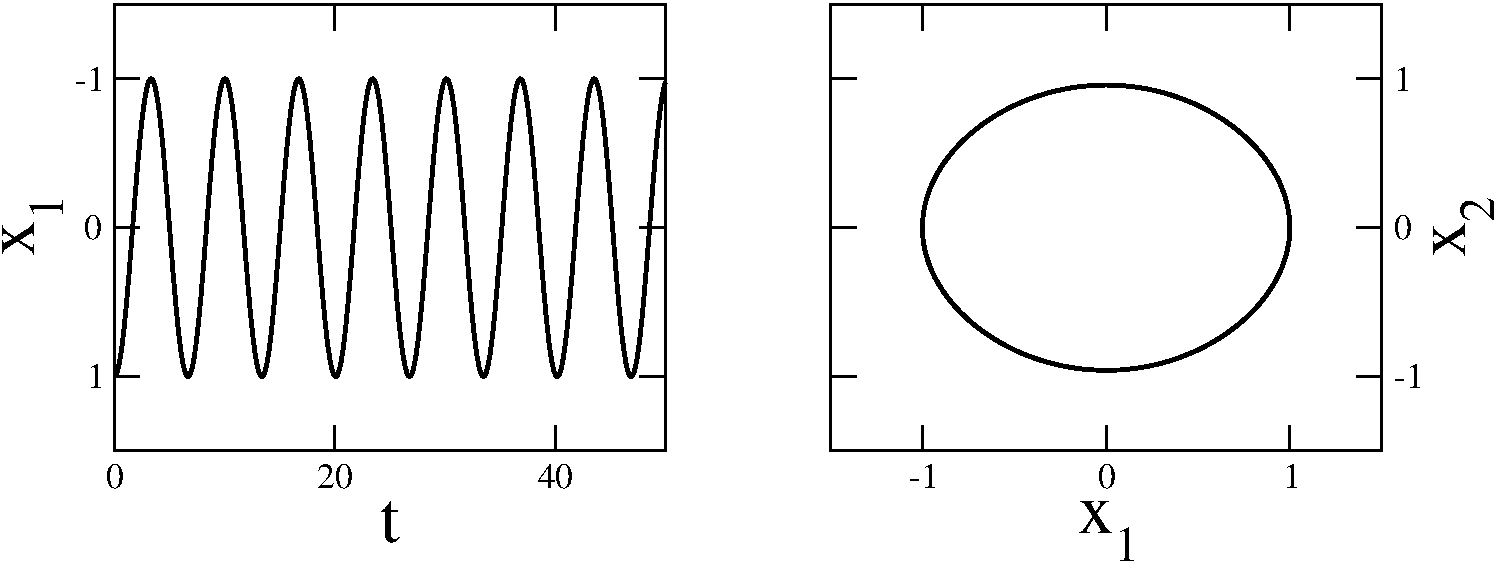
\includegraphics[draft=false,width=1.0\textwidth]{undamped.pdf}}

\vspace{2.5ex}
\centerline{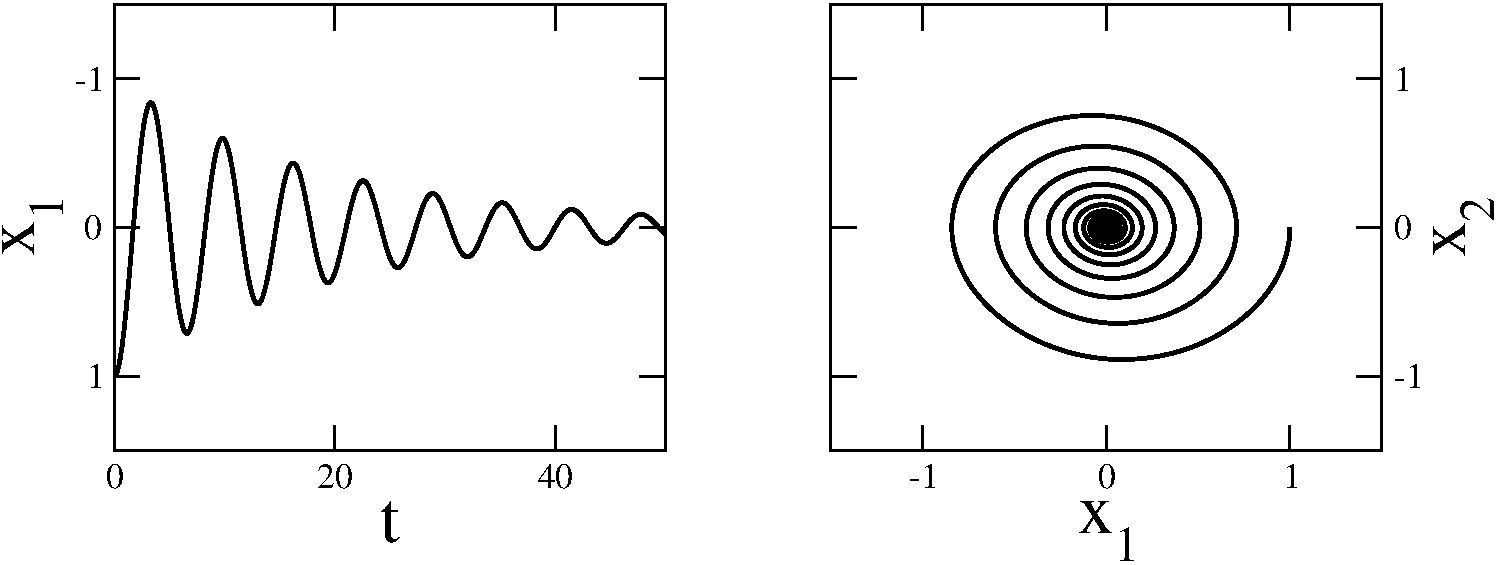
\includegraphics[draft=false,width=1.0\textwidth]{damped.pdf}}

\vspace{2.5ex}
\centerline{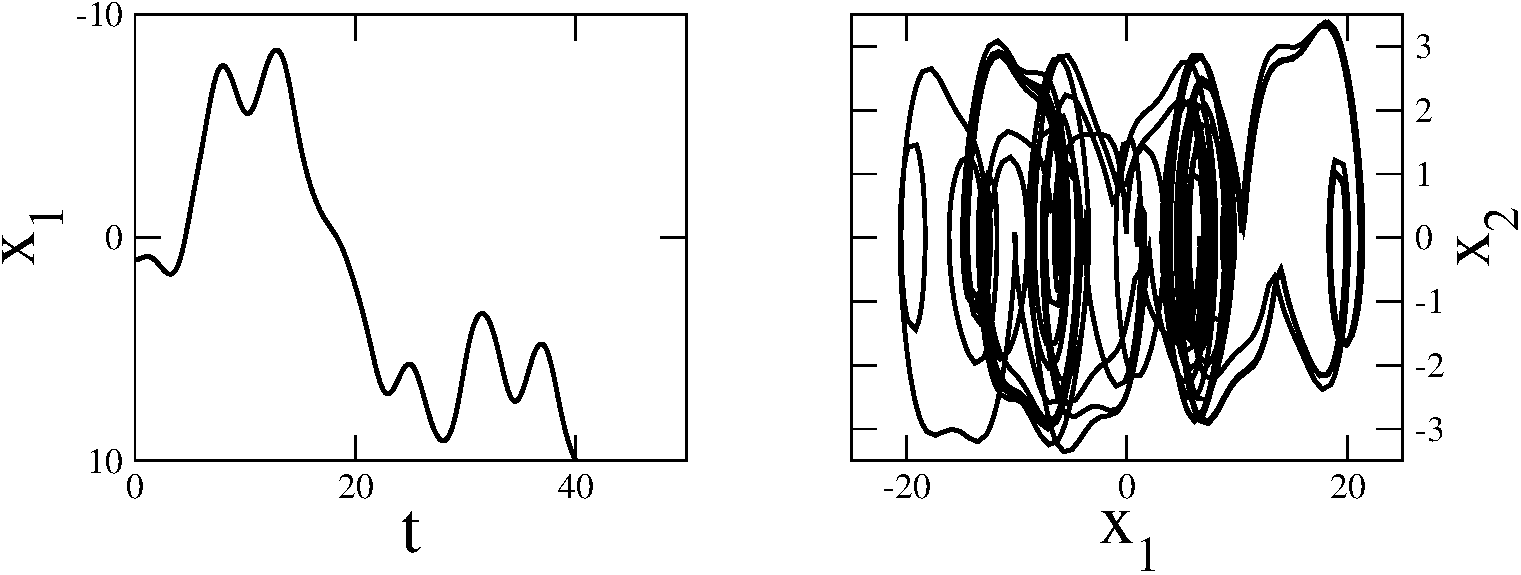
\includegraphics[draft=false,width=1.0\textwidth]{damped_driven.pdf}}
\end{minipage}

\end{frame}





\begin{frame}
 \heading{Steppers -- solvers}

 \vspace{2ex}

 {\bf Stepper Concepts}: Stepper, ErrorStepper, ControlledStepper, DenseOutputStepper

 \vspace{2ex}

 {\bf Stepper types}: 
 \begin{itemize}
  \item Implicit -- {\tt implicit\_euler}, {\tt rosenbrock4}
  \item Symplectic -- {\tt symplectic\_rkn\_sb3a\_mclachlan}
  \item Predictor-Corrector -- {\tt adams\_bashforth\_moulton}
  \item Extrapolation -- {\tt bulirsch\_stoer}
  \item Multistep methods -- {\tt adams\_bashforth\_moulton}
 \end{itemize}

 \vspace{2ex}
 Some of them have step-size control and dense-output!

 \vspace{2ex}

 For details see the odeint documentation!

\end{frame}
